\section{Types of Signals}
%----------------complex exp in ct----------------%
\subsection{Periodic Complex Exponential Signals in Continuous-time Domain}

 \[ x(t) = e^{j\omega_0 t} \]
\begin{itemize}
    \item Periodic, period $T = \frac{2\pi}{\lvert \omega_0 \rvert}$.
    \item The signal $x(t) = e^{-j\omega_o t}$ has the same period.
    \item The complex exponential defined above is closely related to the sinusoidal signal:
 \[ x(t) = A \cos(\omega_0 t + \phi) = \frac{A}{2} e^{j\phi}e^{j \omega_0 t} +\frac{A}{2} e^{-j\phi}e^{-j \omega_0 t} \]
  \ which has the same period $T = \frac{2\pi}{\lvert \omega_0 \rvert}$.
 \item The complex exponentials and sinusoidal signals have \textbf{infinite energy} and \textbf{finite
  power}.
 \begin{itemize}
  \item Example: for the signal $x(t)= A \cos(2\pi \omega_{0}t+\phi)$ with the period $T_{1}$,
  \[ \text{Power} = \frac{A^{2}}{2} \]
 \end{itemize}
\end{itemize}

%----------------complex exp in dt----------------%
\subsection{Periodic Complex Exponential Signals in Discrete-time Domain}

 \[ x[n] = e^{j\omega_0 n} \]
 \ And the sinusoidal signal becomes 
 \[ x[n] = A \cos(\omega_0 n + \phi) = \frac{A}{2} e^{j\phi}e^{j \omega_0 n} +\frac{A}{2} e^{-j\phi}e^{-j
  \omega_0 n} \]
 \begin{itemize}
  \item $n \in \mathbb{Z}$ (\textit{i.e.,} $n$ is an integer). Thus, $x[n]$ is the same signal for $\omega_0 + 2\pi k$ with $k \in
   \mathbb{Z}$. The frequency of oscillation in discrete time exponentials does not increase
   monotonically but is limited to $2\pi$.
  \item $x[n]$ is not always periodic.
 \end{itemize}
 
%----------------unit imp in dt----------------%
\subsection{The Unit Impulse in Discrete-time Domain}

The \textbf{unit impulse function} (or, delta function) defined in the discrete-time domain (\autoref{fig:delta}) is \\
\boxed{
 \begin{minipage}{0.3\textwidth}
   \[  \delta[n] = \begin{cases}
   1,&n=0\\
   0,&n\neq0
  \end{cases}\]
 \end{minipage} \
 \begin{minipage}{0.7\textwidth}
  \begin{figure}[H] 
      \centering 
      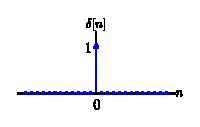
\includegraphics[width=0.5\textwidth]{images/delta_signal.eps}
      \caption{The unit impulse} 
      \label{fig:delta}
  \end{figure}
 \end{minipage}
  }
  
The discrete-time unit impulse \textbf{delayed by an  integer $k$} (\autoref{fig:delta_shift}) is defined as: \\
\boxed{
 \begin{minipage}{0.3\textwidth}
   \[ \delta[n-k] = \begin{cases}
   1,&n=k\\
   0,&n \neq k\\
  \end{cases}\]
 \end{minipage} 
 \begin{minipage}{0.7\textwidth}
  \begin{figure}[H]
      \centering 
      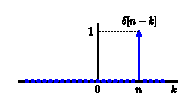
\includegraphics[width=0.5\textwidth]{images/delta_signal_shift.eps}
      \caption{The unit impulse delayed by an integer $k$}
      \label{fig:delta_shift}
      \end{figure}
 \end{minipage}
}

\begin{itemize}
    \item For any discrete-time signal $x[n]$, we have
    \[ x[n] \ \delta[n-k] = x[k] \ \delta[n-k] \]
    \textbf{This implies} any signal multiplied by the unit impulse is zeroed for all time samples, apart from the integer time where the unit impulse is centred.
    
    \item From the property above, we have:
     \begin{align*} 
     \begin{split}
         \sum_{n=-\infty}^{\infty}x[n]\delta[n-k]  
         &= \sum_{n=-\infty}^{\infty}x[k] \ \delta[n-k] \\
         &= x[k] \cancelto{1, \text{when} \ k=n}{\sum_{n=\infty}^{\infty}\delta[n-k]} \\
         &= x[k]
     \end{split} 
     \end{align*}
     
    \item Any arbitrary discrete-time signal can be expressed as the sum of \textbf{scaled} and \textbf{delayed} impulses:
    \[ x[n] = \sum_{k=-\infty}^{+\infty}x[k]\delta[n-k] \] 
\end{itemize}

%----------------unit imp in dt----------------%
\subsection{The Unit Step in Discrete-time Domain}
The \textbf{unit step function} defined in the discrete-time domain (\autoref{fig:discrete_unit_step}) is\\
\boxed{
 \begin{minipage}{0.3\textwidth}
  \[u[n] = \begin{cases}
   1, & n\geq 0\\
   0, & n<0 \\
  \end{cases} = \sum_{k=0}^{+\infty}\delta[n-k] \]
 \end{minipage}
 \begin{minipage}{0.7\textwidth}
  \begin{figure}[H]
      \centering 
      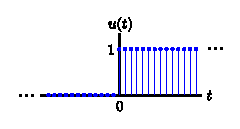
\includegraphics[width=0.6\textwidth]{images/unit_step_discrete.eps}
      \caption{Unit step in discrete-time domain}
      \label{fig:discrete_unit_step}
  \end{figure}
 \end{minipage}
}
\begin{itemize}
    \item The discrete-time unit impulse function is the \textit{derivative} of the discrete-time unit step function.
    \[ \delta[n] = u[n] - u[n-1] \]
\end{itemize}

%----------------unit step in ct----------------%
\subsection{The Unit Step in Continuous-time Domain} 
The \textbf{unit step function} defined in the continuous-time domain (\autoref{fig:continuous_unit_step}) is \\
\boxed{
 \begin{minipage}{0.3\textwidth}
  \[ u(t) = \begin{cases}
   1, & t > 0\\
   0, & t < 0 \\
  \end{cases} \]
 \end{minipage}
 \begin{minipage}{0.7\textwidth}
  \begin{figure}[H]
      \centering 
      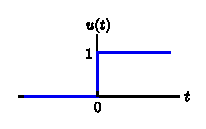
\includegraphics[width=0.5\textwidth]{images/unit_step_continuous.eps}
      \caption{Unit step in continuous-time domain}
      \label{fig:continuous_unit_step}
  \end{figure}
 \end{minipage}
}
\begin{itemize}
    \item The continuous-time unit step function has a discontinuity in $t=0$, hence, it is \textbf{not differentiable}. 
    
    \item The aforementioned issue could be addressed using the concept of \textit{limit}. By expressing the delta function as the derivative of the unit step function over an infinitesimal period of time, $\Delta$, we have
    \[
        \delta_{\Delta}(t) = \frac{\mathrm{d}u_{\Delta}(t)}{\mathrm{d}t} 
    \]
    where
    \begin{itemize}
        \item The area of $\delta_{\Delta}(t)$ equals to 1 at any value of $\Delta$.(\autoref{fig:continuous_unit_step_approx}, right)
        \item As $\Delta \rightarrow 0$, $u_{\Delta}(t) \rightarrow u(t)$. (gradient $\to 0$) (\autoref{fig:continuous_unit_step_approx}, left)
        \item As $\Delta \rightarrow 0$, the impulse $\delta_{\Delta}(t)$ becomes of shorter duration and higher amplitude:$\delta(t) = \lim_{\Delta \to 0} \delta_{\Delta}(t)$
    \end{itemize}
    \begin{figure}[h] 
        \centering 
        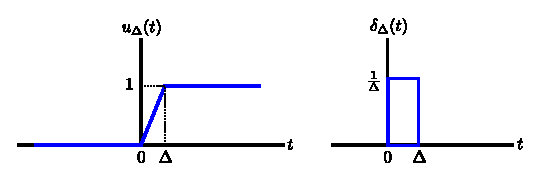
\includegraphics[width=0.8\textwidth]{images/delta_approx.eps}
        \caption{Continuous approximation to unit step}
        \label{fig:continuous_unit_step_approx}
    \end{figure}
    
    \item The unit step function can be reconstructed by integrating the delta function from negative infinity to $t$ (\autoref{fig:unit_step_shift}, left),
    \[
        u(t) = \int_{-\infty}^{t} \delta(\tau) \mathrm{d}\tau
        = 
        \begin{cases}
            1, & t \geq 0 \\
            0, & t < 0 \\
        \end{cases}
    \]
    where $\tau$ is a simply a \textit{dummy} variable used to replace the notation of $t$.
    
    \item for the discrete-time case, the unit impulse in the continuous-time domain can be shifted along the time axis. The unit impulse shifted by the time delay is $\delta(t-\sigma)$.
    
    \begin{figure}[H] 
        \centering
        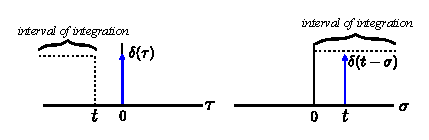
\includegraphics[width=.8\textwidth]{images/unit_step_shift.eps}
        \caption{Unit impulse shifted by the time delay}
        \label{fig:unit_step_shift}
    \end{figure} 
\end{itemize}

 \begin{minipage}{0.5\textwidth}
 \begin{itemize}
\item In continuous-time domain: (similar to discrete-time domain)
\[ x(t)\delta_{\Delta}(t) \approx x(0)\delta_{\Delta}(t) \]
As $\delta_{\Delta}(t)\rightarrow \delta(t)$: better approximation
\[ x(t)\delta(t) = x(0)\delta(t) \]
More generally: with time-shifting
\[ x(t)\delta(t-t_{0}) = x(t_{0})\delta(t-t_{0}) \] 
\end{itemize}
\end{minipage}\hfill
\begin{minipage}{0.5\textwidth} 
    \begin{figure}[H]
    \centering 
    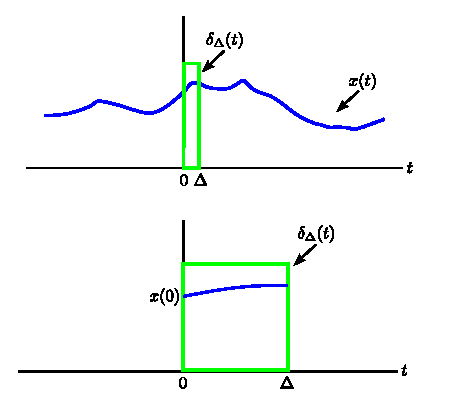
\includegraphics[width=0.9\textwidth]{images/unit_step_continuous_shift.eps}
    \caption{Continuous approximation of the unit impulse} 
\end{figure}
\end{minipage}
 
 \begin{itemize}
\item We also obtain:
\begin{align*}\begin{split}
\int_{-\infty}^{\infty} x(t)\delta(t-t_{0})\mathrm{d}t &= \int_{-\infty}^{\infty} x(t_{0})\delta(t-t_{0})\mathrm{d}t \\
&= x(t_{0})\int_{-\infty}^{\infty} \delta(t-t_{0})\\
&= x(t_{0}) 
\end{split}
\end{align*}
\item This implies that any arbitrary continuous-time signal $x(t)$ can be represent as:
\[ x(t) = \int_{-\infty}^{\infty} x(\tau)\delta(t-\tau)\mathrm{d}\tau \]
%This is similar to another property for discrete-time signals.
\end{itemize}

%----------------Convolution----------------%
\subsubsection{Convolution}
We define the following transformation between two signals (convolution):
\[ y(t) = \int_{-\infty}^{\infty} x(\tau) \ h(t-\tau)\mathrm{d}\tau = x(t)*h(t) \]
\[ y[n] = \sum_{k=-\infty}^{+\infty}x[k] \ h[n-k] = x[n]*h[n] \]
\textit{Convolution in the time main is equivalent to the multiplication in the frequency domain!} \\

For any continuous-time signal and any discrete-time signal:
\[ x(t) = x(t) * \delta(t) \]
\[ x[n] = x[n] * \delta[n] \]
by extension for arbitrary delays:
\[ x(t-t_{0}) = x(t) * \delta(t-t_{0}) \]
\[ x[n-k] = x[n] * \delta[n-k] \]

%----------------summary----------------%
\begin{tcolorbox}[title=Summary of properties of the unit impulse, breakable]
 \begin{itemize}
  \item For \textbf{multiplication}:
   \[ x(0)\cdot \delta(t) = x(t)\cdot \delta(t) \]
   \[ x[0]\cdot \delta[n] = x[n]\cdot \delta[n] \]
\ \\ 
   \[ x(t_{0})\cdot \delta(t-t_{0}) = x(t)\cdot \delta(t-t_{0}) \]
   \[ x[k]\cdot \delta[n-k] = x[n] \cdot \delta[n-k] \]
  \item For \textbf{convolution}:
   \[ x(t) = x(t)*\delta(t) \]
   \[ x[n] = x[n]*\delta[n] \]
\ \\
   \[  x(t-t_{0}) = x(t)* \delta(t-t_{0}) \]
   \[ x[n-k] = x[n]*\delta[n-k] \]
 \end{itemize}
\end{tcolorbox} 

%\subsection{Other Common Signals}
